\documentclass[12pt,letterpaper]{article}
\setcounter{page}{0}

\usepackage{bbm}
\usepackage{hhline}
\usepackage[multiple]{footmisc}
\usepackage{floatpag,amsmath,amsthm,amssymb}
\usepackage{changepage}

% Figure panel header font
\newcommand{\panel}{\fontfamily{phv}\selectfont\scriptsize\textbf}
\usepackage{amsmath} 
\DeclareMathOperator*{\argmin}{arg\,min}
\DeclareMathOperator*{\argmax}{arg\,max}


%%%%%%%%%%%%%%%%%%%%%%%%%%%%%%%
%% LOAD LOCAL COMPILATION PATHS
%%%%%%%%%%%%%%%%%%%%%%%%%%%%%%%
\newcommand{\HOME}{\string~}

% set input paths
\newcommand{\includepath}{.}
\newcommand{\shrugpath}{.}

% include standard package
\usepackage[latin1]{inputenc}
\usepackage{setspace}
\usepackage{amsmath}
\usepackage{amsthm}
\usepackage{amsfonts}
\usepackage{longtable}
\addtolength{\textwidth}{5cm}
\addtolength{\textheight}{5cm}
\usepackage{fullpage}
\usepackage{amssymb}
\usepackage[colorlinks=true]{hyperref}
\usepackage{url}
\usepackage{graphicx}
\usepackage{epstopdf}
\usepackage{multirow}
\usepackage{array}
\usepackage{harvard}
\usepackage{tabularx}
\citationmode{abbr}

\usepackage{float}
% \usepackage{perpage}
% \MakeSorted{figure}
% \MakeSorted{table}
\usepackage{lscape}
\usepackage{verbatim}
\usepackage{pdflscape}
\usepackage{chngcntr}
\usepackage{appendix}
\usepackage{booktabs,calc}
\usepackage{ulem}

% allow yellow highlighting in tables
\usepackage{color,colortbl}
\usepackage{soul}
\definecolor{Yellow}{rgb}{.88,1,.65}
\definecolor{Green}{rgb}{.65,1,.65}
\definecolor{Red}{rgb}{1,.65,.65}

\citationstyle{dcu}

\usepackage[labelfont=bf,center,large,labelsep=newline]{caption}
\usepackage{subfig}
% \counterwithout{subtable}{table}
\def\changemargin#1#2{\list{}{\rightmargin#2\leftmargin#1}\item[]}
\let\endchangemargin=\endlist

% define subscript / superscript commands
\newcommand{\superscript}[1]{\ensuremath{^{\textrm{#1}}}}
\newcommand{\subscript}[1]{\ensuremath{_{\textrm{#1}}}}

% create a shortcut for newlines in captions:
\newcommand{\cnewline}{\hspace{\linewidth}}

%format paper to save trees
\usepackage[right=1in,left=1in,top=1in,bottom=1in]{geometry}
\usepackage{savetrees}

%AER style headers
\def\thesection{\arabic{section}}
\def\thesubsection {\thesection.\arabic{subsection}}

% set home path
\newcommand{\HOME}{\string~}


% disable hyperlinks, which were breaking on appendix references
\usepackage[options]{nohyperref}

\title{Development Research at High Geographic Resolution: \\ An
  Analysis of Night Lights, Firms, and Poverty in India \\ using the
  SHRUG Open Data Platform\footnote{Sam Asher (corresponding author)
    is assistant professor of international economics at Johns Hopkins
    SAIS and co-founder of the Development Data Lab; his email address
    is sasher@jhu.edu. Tobias Lunt is chief data scientist and
    co-founder of the Development Data Lab; his email is
    lunt@devdatalab.org. Ryu Matsuura is a PhD student in economics at
    Northwestern University; his email address is
    ryumatsuura@u.northwestern.edu. Paul Novosad (corresponding
    author) is associate professor of economics at Dartmouth College
    and co-founder of the Development Data Lab; his email address is
    paul.novosad@dartmouth.edu. Thanks to Teevrat Garg, Francesca
    Jensenius, Dan Keniston, and Nishith Prakash for sharing data that
    contributed to this dataset. This project and underlying data
    platform were funded by Emergent Ventures. Early work on this
    project was supported by the IGC (project 89414), and a project
    funded by the UK Department for International Development (DFID)
    and the Institute for the Study of Labor (IZA) for the benefit of
    developing countries. All errors are our own. The SHRUG dataset
    can be downloaded at
    \href{http://devdatalab.org/shrug}{http://devdatalab.org/shrug}. A
    supplementary online appendix for this article can be found at The
    World Bank Economic Review website.}}

\author{ Sam Asher \\ Tobias Lunt \\ Ryu Matsuura \\ Paul Novosad \\ }

%%%%%%%%%%%%%%%%%%%%%% 
% TITLE PAGE
%%%%%%%%%%%%%%%%%%%%%% 
\begin{document}
\date{January 2021}
\maketitle
% JEL CODES 
% R11 -- Regional Economic Activity: Growth, Development, Environmental Issues, and Changes
% C81 -- Methodology for Collecting, Estimating, and Organizing Microeconomic Data
% O12 -- Microeconomic Analyses of Economic Development

\begin{abstract}

The SHRUG is an open data platform describing multidimensional
socioeconomic development across 600,000 villages and towns in
India. This paper presents three illustrative analyses only possible
with high-resolution data. First, it confirms that nighttime lights
are highly significant proxies for population, employment, per-capita
consumption, and electrification at very local levels. However,
elasticities between night lights and these variables are far lower in
time series than in cross section, and vary widely across context and
level of aggregation. Next, this study shows that the distribution of
manufacturing employment across villages follows a power law: the
majority of rural Indians have considerably less access to
manufacturing employment than is suggested by aggregate data. Third, a
poverty mapping exercise explores local heterogeneity in living
standards and estimates the potential targeting improvement from
allocating programs at the village- rather than at the
district-level. The SHRUG can serve as a model for open
high-resolution data in developing countries.
  
\\ JEL Codes: R11/C81/O12
\\ Keywords: open data, big data, administrative data, nighttime lights, poverty, India
\end{abstract}

\newpage
\clearpage
\setcounter{pag}{1} \doublespacing
\section{Introduction}
\label{sec:intro}

Development and economic growth, insofar as they affect the living
standards of individuals, are highly localized phenomena. Employment
opportunities, schools, public goods, and welfare schemes are relevant
to individuals primarily if they are accessible within a short
distance. However, due to the nature of data available to researchers,
analysis of development has largely occurred at an aggregate
geographic scale. In India, much policy and research has been based on
the National Sample Surveys, which have tracked socioeconomic change
at the district level since independence. But a single Indian district
is home to around 2 million people, often with vast variation in
living standards. This variation is demonstrated in
Table~\ref{tab:var_decomp_panel}, which shows the share of variation
in various development outcomes at different levels of geographic
variation. 55\% of variation in mean village per capita consumption
and over 95\% of variation in rural non-farm employment occurs below
the district level. The National Sample Surveys often base district
statistics on fewer than 100 households per district, missing much of
this microgeographic variation. 

The computerization of government administration and the proliferation
of new data sources such as satellite imagery has provided researchers
with the opportunity to study development at higher geographic
resolution than ever before. However, it has been enormously costly
and time-consuming to discover, obtain, clean, and merge data sources
that were not designed for social science research. When researchers
do pay the fixed costs, it is often difficult for other research teams
to make use of that data; despite recent efforts to make data
availability a key part of the publication process, published data is
rarely comprehensive or easily linked to other data sources. The high
fixed costs of making use of new data is particularly harmful to
researchers lacking the funding and time to make major investments in
data assembly, such as many doctoral students and researchers in the
very countries that development economics seeks to study.

This paper introduces the Socioeconomic High-resolution Rural-Urban
Geographic Dataset on India (SHRUG), a multidimensional socioeconomic
data platform with high geographic resolution data on demography,
non-farm employment structure, political outcomes, forest cover, night
lights, and administrative program operation, among other dimensions,
for the universe of municipalities (towns and villages) and
legislative constituencies in India from 1990 to 2018 (see Table
\ref{tab:contents}).\footnote{Villages (rural, median population 832)
  and towns (urban, median population 14,684) are the lowest level for
  which the Population Census and many other datasets make data
  available. The lowest level of government in India is comprised of
  urban local bodies for towns, and rural panchayats, which are on
  average comprised of 2--3 villages. Legislative constituencies are
  geographic areas, usually comprised of multiple towns and villages,
  that send one representative each to India's Vidhan Sabhas (state
  legislatures).} The SHRUG is an open dataset but also an open data
platform that is structured to facilitate and encourage sharing of
readily linkable data between researchers in the future.

In this paper, we present three analyses that shed light on the
distribution of economic opportunity within highly localized regions,
analyses that are only possible with high resolution data like the
SHRUG.

We begin by examining the effectiveness of nighttime lights as a
measure of local development. Nighttime lights, as measured from outer
space, have been widely used in recent years to examine patterns of
development in places where local economic data is not
available. Nighttime lights are particularly used in analyses of
programs which have geographic variation which is more precise than
what can be observed in aggregate data; the ability to observe an
economic outcome in a 1km x 1km cell is a key comparative advantage of
night lights. Given the lack of high-precision economic data in most
developing countries, the assumption that night lights have the same
elasticities at both very high and very low levels of geographic
aggregation with a range of outcome variables is largely
untested.\footnote{\citeasnoun{henderson2009b} show that elasticities
  are similar across countries and across large regions within
  countries, but they do not measure elasticities at finer geographic
  levels. And yet the primary use of night lights in research is
  precisely to generate outcome variables at very high geographic
  resolution.}

Our results confirm that night lights are a highly statistically
significant log-linear proxy for a range of development
outcomes---population, employment, per capita consumption, and
electrification---at a very narrow geographical level, even in
specifications with regional fixed effects, in the both the cross
section and in the time series. However, there are two significant
caveats. First, because night lights have independent correlations
with each of these outcomes, it is difficult to tell from night lights
alone which of these proxy variables are being measured. Researchers
have used night lights as a proxy for GDP growth, cross-sectional GDP,
urban extent, public expenditure, and electricity supply and demand,
among other variables
\cite{henderson2009b,baum-snow2012,bleakley2012,min2013,hodler2014,baskaran2015,burlig2016,harari2020,mahadevan2020}. Our
results suggest that all of these proxies are valid, but researchers
have no guarantee that night lights are proxying the specific variable
that they would like to measure and not a different one.

Second, we find that night light elasticities vary substantially
across the level of geographic aggregation and across
contexts. Importantly, we find that night light elasticities are an
order of magnitude smaller in the time series than they are in the
cross section. Night light elasticities with most variables are also
considerably higher in electrified villages than in non-electrified
villages. This finding suggests that researchers should use extreme
caution in applying regional luminosity-to-GDP elasticities from the
literature to microgeographic contexts without additional information,
because these elasticities may be wildly different. Applying
cross-sectional elasticities to time series night light coefficients
is likely to result in a substantial upward bias on GDP estimates.

Moving beyond night lights, we next examine the distribution of
manufacturing and services employment across space. Economic activity
is often highly agglomerated and firm size distributions are known to
follow power laws \cite{ellison1997,gabaix2016}. The amount of
concentration affects the extent to which regional averages reflect
the access to opportunity of the majority of a region's residents. We
show that the distribution of firms across space also follows a power
law, such that some regions have orders of magnitudes more employment
density than others. The extent of employment concentration is higher
for manufacturing than for services firms, and the highest by far for
manufacturing employment in rural areas. The mean Indian village has
15 manufacturing jobs per 1000 people, but the median has less than
5. Almost 80\% of rural Indians live in villages with fewer
manufacturing job opportunities than the rural mean. Regional
employment opportunities, especially for women, may be of limited
relevance if they are not geographically proximate. This analysis
demonstrates that analysis of employment at aggregate geographic
scales may fail to register the lack of labor market opportunities for
most rural workers.

Finally, we conduct a poverty mapping exercise, considering the
problem of a policymaker targeting a program to poor geographic
regions
\cite{ravallion1993,baker1994,bigman2000,bigman2002,elbers2007,brown2019}. We
measure the efficiency gain that could arise from the ability to
allocate a program reaching 25\% of the population at increasingly
finer geography. If the policy-maker can observe poverty only at the
district level (n=618), then allocating the program to the poorest
districts would cover 37\% of the rural poor. Allocating the same
program at the village level would cover 44\% of the rural poor. There
is likely a tradeoff between precise geographic targeting and
administrative cost; highly localized data makes it possible to
estimate the parameters of this tradeoff.

The SHRUG has a number of strengths and weaknesses as an analytic
platform. Its primary strengths are its geographic resolution and
consistent location identifiers over a period of dramatic economic
change. There are few other data sources in developing countries that
allow tracking of public goods, economic activity, politician
characteristics, election results, and many other outcomes at the
village and town level for almost 600,000 consistently-bounded
geographic units.\footnote{There are approximately 605,000 towns and
  villages in India. We collapse these to about 590,000 unique,
  consistent locations that can be tracked over time.} The key
comparative disadvantages of the SHRUG are that (i) most of the
underlying data sources are based on narrow surveys with a few dozen
questions rather than hundreds; and (ii) the SHRUG describes
locational aggregates, rather than individual or firm
microdata.\footnote{Note that it can be rapidly linked to firm-level
  data in the Economic Census, which is openly available.}
Researchers interested in detailed characteristics of individual
households and firms may thus be better served by traditional data
sources.

There are a number of contexts in which the SHRUG may have a comparative advantage:
\begin{itemize}
\item Programs with highly local variation are difficult to evaluate with aggregate data. Examples of analysis of such programs using administrative data (some of which are now in the SHRUG) include \citeasnoun{lehne2016}, \citeasnoun{chhibber2016}, \citeasnoun{burlig2016}, \citeasnoun{an2017pols}, \citeasnoun{aan2019dise}, \citeasnoun{an2019pmgsy}, and \citeasnoun{muralidharan2017}.
\item Analysis at the city/town and legislative constituency level is challenging because neither of these units are identified in India's conventional data sources. SHRUG data are aggregated to both of these levels.
\item Researchers running field experiments typically use national population censuses as sampling frames for new field experiments, but have limited additional data on sample locations before collecting their own baseline surveys. The SHRUG increases the scope of what is known at a local level. Field experimentalists can begin to test for divergent trends in field locations even before conducting a baseline survey.
\end{itemize}

Most of the data underlying both the SHRUG and the papers using
administrative data described above are public. The primary constraint
to using data like these is the time input required to assemble,
clean, and match them to other data sources. The returns to this
activity are increasing in the number of other localized data sources
that they can be matched to. We therefore hope that the existence of
the SHRUG makes it worthwhile for researchers to assemble and share
other administrative and microgeographic datasets describing
additional dimensions of development in India.

We structured the SHRUG to maximize the ease and benefit to
researchers of sharing new data. First, by providing a broad spectrum
of data under a consistent set of identifiers, we hope to create a
standard set of location identifiers for India. Such standardization
can lower the cost of merging datasets for all researchers. Second, we
have structured downloads from the SHRUG to credit individual
contributors. When researchers download data from the SHRUG, they are
asked to cite the authors who created each component of the SHRUG that
they are using.\footnote{For instance, users of the data in the SHRUG
  on the criminal charges facing Members of Legislative Assemblies
  should cite \citeasnoun{prakash2014}.} This citation structure is
intended to give researchers an incentive to contribute, because clean
data integrated into the SHRUG will receive more users and generate
more citations than data on journal web sites that are suitable for
replication only.\footnote{The present version of SHRUG already
  includes contributions from two groups of researchers other than
  ourselves. Since making the data public in September 2019, three
  additional groups of researchers are working on additional data
  sources that they plan to integrate with the SHRUG.}

Finally, SHRUG data are released to non-commercial users under a
copyleft license (the Open Database License, or ODbL), which commits
researchers who link the SHRUG to non-proprietary data to also post
that non-proprietary data in a complete form with SHRUG identifiers at
the time that their research is published.\footnote{More information
  on the ODbL is available at
  \href{https://opendatacommons.org/licenses/odbl/index.html}{https://opendatacommons.org/licenses/odbl/index.html}.}
Given the long publication lags in economics, this license gives
researchers ample lead time to work on additional projects with the
data that they have collected, but commits them to sharing data in a
reasonable time horizon. Like the limited protection time offered by a
patent, this approach trades off the private incentive to researchers
of developing unique data sources with the much greater public good of
making those data sources available to the full network of researchers
that can make use of them.\footnote{Data under formal proprietary
  contracts that restrict sharing are excluded from this commitment at
  this time.}

The current release of the SHRUG (version 1.5) describes: (i)
demographic and public goods data on every town and village in India
from 1991 to 2011; (ii) employment and location of every non-farm firm
in India from 1990 to 2013; (iii) legislative election results from
1980 to 2018 \cite{Jensenius2017}; (iv) assets, liabilities, and
criminal charges of all politicians in office and many additional
candidates from 2004 to 2017 \cite{prakash2014}; (v) remotely sensed
night lights from 1994 to 2013; (vi) remotely sensed forest cover from
2000 to 2019; (vii) the share of labor force in agriculture and small
area estimates of consumption from the Socioeconomic and Caste Census
of 2012; and (viii) administrative data from the implementation of
India's national rural roads program. As new census, remote sensing,
and administrative datasets are released, the breadth of this panel
will continue to grow.

This paper first describes the construction of the SHRUG in some
detail in Section~\ref{sec:data}, along with several validation
exercises. Section~\ref{sec:results} presents the analyses of night
lights, agglomeration, and poverty. Section~\ref{sec:strengths}
discusses the strengths and weaknesses of the SHRUG as an analytical
tool. Section~\ref{sec:conc} concludes with a discussion of the
copyleft license and framework for improving institutions of data
sharing between researchers.

\section{Data: A 25-year Multidimensional Panel of Locations}
\label{sec:data}

All variables in SHRUG are disaggregated to the level of the village
(n=590,648), the town (7528), and the state legislative constituency
(n=2800), covering the entire country. The different components are
summarized briefly in Table~\ref{tab:contents} and in detail in the
SHRUG metadata table.\footnote{The SHRUG metadata table can be found
  at
  \href{devdatalab.org/shrug-metadata}{devdatalab.org/shrug-metadata}.}

All of these data sources were initially generated with diverse
geographic identifiers which were not straightforward to link. The
Population and Economic Censuses are published with town and village
codes with incomplete correspondences across different rounds. PMGSY
data is published at the habitation level; most villages consists of
between one and three habitations. Remote sensing data is published in
grid cells, while political data is published at the constituency
level; constituencies are approximately the size of subdistricts (a
standard unit in the Population Censuses), but with different and
overlapping boundaries.

Any pair of these datasets can be reconciled and matched to each
other, albeit with significant labor input. Sources of information
used to match data include numeric identifiers, names, maps, data
contents, and external data sources. In most cases, none of these
information sources provide a perfect match. Identifiers are rarely
consistent across datasets; sometimes they are consistent across some
states but not others. Locations may be known by multiple names, and
names may change over time; they virtually always have different
spellings across and even within data sources. Maps are supplied with
different projections and different degrees of error; boundaries which
should be identical in different mapping sources often are
not. Locations themselves change, splitting, merging, and realigning
boundaries in complex ways.

The process of matching these datasets consists of developing
algorithms to use as many of these information sources as possible,
and then tuning those algorithms based on manual verification of
samples of data. Individual verification of every match is however not
feasible when observations number in the hundreds of thousands. Some
units cannot be matched even with manual verification because there is
insufficient information available. Some degree of incorrect matches
are inevitable.

The core contribution of the SHRUG is a set of universal location
identifiers (one at the town and village level, and one at the
constituency level) that span the entire sample period from
1990--2018. All of the datasets above can be rapidly linked to these
identifiers in every period. When using the SHRUG, linking disparate
data sources takes seconds rather than months. By releasing the data
with these universal identifiers, our hope is to make them a standard
for economic research in India, allowing future data sources to be
linked to the data sources described here with ease.

This section describes the process of creating the universal
identifiers that are at the heart of the SHRUG. The definitions of
individual data fields are described in detail in the SHRUG
codebook.\footnote{The SHRUG codebook can be found at
  \href{http://www.devdatalab.org/shrug}{http://www.devdatalab.org/shrug}.}

To keep its size reasonable, the SHRUG 1.5 data package includes only
a subset of the fields in the Economic and Population Censuses. We
provide linking keys to each of these source datasets to make it easy
for users to bring in additional fields from these open data sources.

\subsection*{Building the Town and Village SHRUG}

The key challenge in creating time series administrative data in India
is in dealing with changing unit boundaries. Faced with the challenge
of villages being split, merged, and integrated with cities and towns,
the decennial Census has opted to create new location identifiers in
every decade since 1991. Further complicating the process of matching
locations over time, district boundaries have changed substantially,
with hundreds of new districts created between 1991 and 2011.  The
Census provides digital keys to link villages and towns to prior
censuses, but they are highly incomplete. The Census district
handbooks contain detailed descriptions of boundary changes in
narrative format only. All of these sources have errors and
inconsistencies.

We used both the digital linking keys and the district handbooks to
create the best possible correspondence of villages and towns across
the 1991, 2001, and 2011 censuses.\footnote{The Census District
  Handbook is a 500+ page book describing all changes to boundaries in
  a given census district in each intercensal period. There is one
  book like this for each of India's $\sim$700 districts.} We
supplemented this with a custom fuzzy string matching program to match
village and town names over time.\footnote{The program is called
  masala-merge and is available at
  \href{http://github.com/devdatalab/masala-merge}{http://github.org/devdatalab/masala-merge}. It
  performs a Levenshtein string match, customized for common string
  substitutions used in Indian languages.}  We conducted a hierarchical
match from the largest to the smallest administrative units. We began
with a match of districts across Population Censuses. A 1991--2001
district correspondence was shared with us by
\citeasnoun{kumar2015}. We constructed the 2001--2011 district match
based on the back-referenced village identifiers in the 2011 census,
which provided a 2001 census village identifier for the majority of
2011 villages. Within districts, we then matched subdistricts on the
basis of names where possible, and then we matched villages within
subdistricts, again on the basis of names. Where the district and
subdistrict maps indicated substantial changes in district and
subdistrict boundaries, we matched villages and towns within
higher-level aggregates of districts and subdistricts.  We validated
the data using internal consistency checks and data from multiple
sources, including geospatial village and town data assembled by other
research groups. Appendix Table~S1
(available at \emph{The World Bank Economic Review} website)
summarizes the share of population from each Population Census that is
matched at the village and town level to the SHRUG by state. Virtually
all towns and villages were matched across the census periods: the
match rates is 98\% or higher for all but two small states in 1991.

To match the Economic Censuses to the Population Censuses, we used the
location directories for 1998 and 2005, which were shared with us by
the Ministry of Statistics (MOSPI).  For 2013, we used the fact that
the Economic Census location codes corresponded to the Population
Census short codes, which were available with village and town names
on the Population Census website. The final step in all these cases
was a match using location names with the algorithm described above.

MOSPI was not able to provide a location directory for the 1990
Economic Census. The EC district codes were the same as those used in
the 1991 Population Census, but the lower level codes were different
in some states. We worked with MOSPI to identify the set of states
that used the same identifiers in the 1991 Population Census and the
1990 Economic Census. It was straightforward in the data to
distinguish these states from the ones which created new codes, and we
matched villages and towns on the basis of identifiers in these
places. For towns that could not be reliably matched on the basis of
the town codes, we obtained a number of additional matches in
situations where three conditions all held: (i) towns could be
uniquely matched within districts to the 1991 Population Census based
on the number of wards;\footnote{For instance, if a district had two
  towns in the 1991 Population Census, with respectively four and
  seven wards, we matched them to the 1990 Economic Census towns with
  the same number of wards.} (ii) their within-district size rank was
the same in the Economic and Population Censuses; and (iii) the number
of people per Economic Census job was within an order of magnitude of
the dataset mean, which was approximately 20. Appendix
Table~S2 summarizes the share of employment
in each Economic Census that is matched to the SHRUG, by
state. Because of the absence of the 1990 location directory, the
match rate for the 1990 Economic Census is much lower than for the
other censuses.

Additional administrative datasets (such as the PMGSY road data and
the Socioeconomic and Caste Census) were matched using a similar
approach. These matches are described in more detail in
\citeasnoun{an2019pmgsy}.

Location splitting and merging over time results in an inordinately
complex set of linking keys. To create a dataset that was unique on
the same locations for all of the different underlying data sources,
we aggregated location units until a set of boundaries could be found
that was unique across all years. We gave each of these units a unique
SHRUG identifier, or a \textit{shrid}.

A shrid describes a geographical unit that can be mapped consistently across all rounds of the Indian Population and Economic Censuses from 1990 to 2013. In the majority of cases, a shrid describes a single village or town. When villages or towns have merged or separated in the sample period, we have aggregated them in the periods where they appear separately, such that the aggregation is represented by a single consistent shrid in all of the data. Some shrids are thus composed of multiple Population Census villages or towns, or a combination of villages and towns.

In some cases, village and town boundaries have changed so dramatically that the aggregated constant boundary unit is quite large. In the case of New Delhi and Chandigarh, whose internal boundaries have changed frequently since 1991, the shrid is the entire city-state. In the case of Mumbai, a shrid is a district, which is the smallest non-changing unit. Creating time-consistent data within urban boundaries is a challenging and distinct project which we are also working on, but is beyond the scope of this iteration of the SHRUG.

The use of a single consistent unit for each geographic location is a critical simplification for the researcher. Without a one-to-one relationship between locations across datasets, each additional bilateral merge requires an increasingly complex task of handling splits, joins, and unit duplications. When working with shrids, any number of datasets can be merged without increasing complexity.

The complete keys linking shrids to their original population and Economic Census codes and location names are posted with the SHRUG, making it easy to bring in additional data that is already linked to Population Census codes. As described in the codebook, we have designed a naming convention for shrids that will be forward-compatible with future censuses as well. New keys will be posted as future censuses are released.

\subsection*{Creating a Constituency-Level Panel}

The boundaries of India's 543 parliamentary and some 4000 legislative constituencies do not align with the aggregate administrative boundaries used by India's data collection agencies. To create a constituency-level dataset with economic outcomes, we matched villages and towns to constituencies using digital maps and collapsed the data to the legislative boundaries.\footnote{SHRUG 1.5 does not include electoral data for parliamentary constituencies or panchayats, but these will be included in the future. Boundary data was obtained from ML Infomap.} We created a set of time-invariant constituency identifiers for the 3rd and 4th delimitations.\footnote{This was necessary because the Election Commission of India (ECI) does not always use consistent numeric identifiers over time. The keys provided with the constituency-level data make it possible to link to the ECI data and thus to any other dataset that uses those identifiers.}

Creating a constituency-level panel from town and village microdata poses a number of challenges.  First, because of the fuzzy matching process, there are some villages which were matched to some Censuses and not to others. Simply aggregating employment in matched villages to the constituency level would thus overstate employment gain in constituencies that have improving match rates over time. We corrected these errors with an imputation process which we describe here.

In the 2011 Population Census, we have matched 100\% of towns and
villages to constituencies, while the match rates in 1991 and 2001 are
very high but imperfect. For each constituency, we therefore know the
2011 population in towns and villages that were matched to the other
censuses, and the 2011 population in towns and villages that were not
matched. We impute the prior years' population in unmatched locations
by assuming that the within-constituency 2001--2011 population growth
rate is the same in towns and villages that we did \textit{not} match
in 2001 as it is in the towns and villages that we \textit{did}
match. We can repeat the process to obtain the full set of populations
in 1991. Because the match rates in 1991 and 2001 are so high, any
error in this imputation process is likely to be minimal. This process
will cause the aggregated constituency population to be closer to the
truth than if we counted missing locations as having zero population.

We repeated the process to aggregate the employment count in the
Economic Censuses, and the public goods counts in the Town and Village
Directories. For each Economic Census, we assumed that the
employment-to-population ratio for missing locations is the same as it
is for non-missing locations within the same constituency. For
location amenities that are aggregated with means rather than sums
(such as the mean number of hours of electricity), we generated an
aggregate based on the population-weighted mean in non-missing
locations. To avoid excess dependence on imputed values, we set fields
to missing in constituencies where locations covering more than 25\%
of the population would be imputed. This means that different
constituencies may be missing different fields depending on the
underlying structure of the data.

Appendix~Figure~S1 runs a simulation to calculate
error rates associated with the imputation process. We randomly drop
additional locations from the 2001 Population Census and then compare
the calculated constituency population to what would be observed if no
locations were dropped. When 25\% of shrids are dropped (the upper
limit of what we include in the data), the average constituency
population is within 2\% of the true value with a slightly negative
bias of 0.015\%.\footnote{Imputed values for constituencies with high
  imputation rates are available from the authors, as is the share of
  imputed data in each constituency-field. These are not included in
  the online SHRUG package because the files are extremely large and
  have relatively narrow usefulness. While it would be desirable to
  use these values to econometrically adjust for the partial
  imputation that took place in calculating these values to adjust for
  the partial imputation of some constituency values, we are not aware
  of an out-of-the-box method that is well-matched to this partial
  imputation structure. The simulated error rates suggest that this
  source of error is small relative to other sources of error in the
  collection of administrative data in India, and thus not a major
  concern.} It is important to note that this imputation process
applies only to the constituency-level data; when Economic or
Population Census data are missing in the town and village data, they
are reported as missing in the SHRUG.

Another challenge that arises is that the available polygon shapefiles
for constituencies and towns/villages are not perfectly aligned, even
though they all use the same WGS84 projection and were obtained from
the same firm. The misalignment is small---on the order of several
hundred meters in the worst cases---but it is enough that some
villages and towns cannot be unambiguously assigned to a single
constituency. We dropped constituencies in which more than 25\% of
2011 population is in villages or towns that cannot be decisively
assigned. We have explored several alternate sources of data and
spoken with several other experts on Indian spatial data, and to our
knowledge there are currently no higher accuracy shapefiles than
these, so this amount of error is unavoidable. There are several
ongoing projects to assign villages to constituencies by digitizing
electoral rolls; as these data become available, we aim to integrate
them into future versions of the SHRUG.

A third challenge is that some towns contain multiple
constituencies. Because the Population Censuses do not report
consistent identifiers at the ward level or below, it is difficult to
identify the population or other characteristics of these
constituencies --- we know only the aggregate population of the
combined constituencies.\footnote{The Population Census reports data
  at the ward level, but the wards change across rounds and do not
  necessarily share boundaries with constituencies.} We therefore
exclude constituencies that include any part of towns that cross
constituency boundaries. Constituencies in large urban areas are
therefore missing population and economic data in the SHRUG. However,
the election and remote sensing measures are included for all villages
because they are not aggregated from village and town data.

The \textit{constituency} SHRUG is therefore not representative --- in
particular, it excludes large cities. However, we are not aware of
other research that measures or exploits socioeconomic data at the
constituency level for large urban constituencies (other than the
remote sensing measures described above), presumably due to the same
boundary misalignment issues that we face here. Constructing such a
dataset using ward maps for India's largest cities would be a valuable
contribution that would enable better study of politics in India's
growing cities.

Finally, India periodically redraws constituencies to account for
population changes. The third delimitation came into effect in 1976
and the fourth in 2008, in the middle of the period covered by the
SHRUG \cite{Iyer2013}. This is not a problem for data construction,
since constituencies are simply defined as polygons. We therefore
match both sets of polygons to villages/towns and create separate
complete constituency-level panels from 1990--2018 for the old and the
new constituency delimitations. Researchers can thus make their own
decisions regarding which polygons to use for which periods. We
provide separate identifiers for the third and fourth delimitations;
there is no correspondence between these as nearly all of the
constituency boundaries were changed.

\subsection*{Remote Sensing Data}

At present, SHRUG includes data from two remote sensing sources:
nighttime luminosity \cite{henderson2009b} and forest cover
\cite{agn2019deforest,townshend2011}. Nighttime luminosity data are
from the National Oceanic and Atmospheric Administration (NOAA), and
provide a luminosity value from 0--63 for each 1 km x 1 km grid
cell. Forest cover data comes from Vegetation Continuous Fields (VCF),
a MODIS product that measures tree cover at a 250m resolution from
2000 to 2019. VCF is predicted from a machine learning algorithm based
on broad spectrum satellite images and trained with human-categorized
data, which can distinguish between crops, plantations and primary
forest cover.

Gridded data from both of these sources were matched and aggregated to
village, town, and constituency boundaries. About 90\% of towns and
villages were georeferenced with polygons, permitting accurate
measurement of night lights and forest cover. About 10\% of locations,
especially in the Northeast, were georeferenced in the mapping data
only by points; we constructed Thiessen polygons to match these to the
forest cover and night light rasters. Locations mapped with Thiessen
polygons are flagged in the data.

\subsection*{Imputation of Consumption Expenditure}
\label{sec:data_cons}

We created a measure of village- and town-level consumption expenditure using data from the Socioeconomic and Caste Census (SECC), a universal enumeration of household assets conducted in 2012. Asset censuses like this are commissioned by the federal government approximately every decade to determine individual eligibility for means-tested poverty relief programs. The SECC enumerates a list of household assets that can be rapidly assessed (including roof and wall material, number of rooms, and assets such as agricultural equipment, vehicles and mobile phones).

We used this asset data to generate small area estimates of
consumption expenditure, following the method of
\citeasnoun{elbers2003}. Using the 2011--2012 IHDS-II (Indian Human
Development Survey, 2011--12, available at
\url{https://ihds.umd.edu}), we regressed total household consumption
on a set of continuous and dummy variables that are equivalent to all
asset and earnings information contained in the SECC. We then used the
coefficients (shown in Appendix~Tables~S3 and S4) to predict household-level consumption in
the SECC microdata. We aggregate this to create a village- and
town-level measure of annual per capita consumption
expenditure. Because the urban and rural asset lists are different, we
use separate estimations depending on whether households were
identified as rural or urban in the SECC.\footnote{The coefficients
  from the model that generate these consumption numbers are estimated
  with statistical error. To allow researchers to account for these
  errors, we used a bootstrap approach, drawing households from IHDS
  with replacement and re-estimating village-level per capita
  consumption 1000 times. These 1000 draws are available as a SHRUG
  package for download and reflect the distribution of per capita
  consumption that arises from the first-stage estimation
  process. Researchers can use these 1000 draws in a second bootstrap
  process to account for the consumption estimation error. The Data
  Appendix in \citeasnoun{an2019pmgsy} describes this process in
  additional detail.} Village- and town-level asset ownership shares
are also available in the house listing for the 2011 Population Census
and match the asset shares in the SHRUG closely.

In addition to average per capita consumption, we included the share of individuals in each town and village who live in households with per capita consumption below the 2012 national poverty rate, defined in two ways: below \$2, or below Rs. 27.2 per day in villages and Rs. 33.33 in cities and towns.\footnote{\$2 threshold converted in PPP to Indian rupees in the following way. It should be noted that GDP per capita (current US\$) of India in 2012 is 1,446.985, GDP per capita PPP of India in 2012 is 4,916.486, and exchange rate between Indian rupee and US\$ in 2012 is 53.427 according to the World Bank. Thus, \$2 PPP is equal to 31 rupees $(2 * 1,446.985 / 4,916.486 * 53.427)$ or 31 rupees per day. 27.2/33.33 rural/urban classification is from the 2011 Suresh Tendulkar Committee report \cite{planningcommissionofindia2009}.}

We have validated these consumption estimates in three ways. First, we
affirmed that the consumption distribution broadly matches the
2011--12 IHDS and 2012 NSS. The consumption distribution in each
dataset is shown in Figure~\ref{fig:ihds_nss_shrug_cons_kdensity}. For
the sake of comparability, the locations used are Population Census
villages in the SHRUG and the closest analog in the other two datasets
(first stage unit in the NSS and primary sampling unit in the
IHDS).\footnote{Each observation in this density plot is a
  village. For the sample surveys, we apply sampling weights when
  calculating village means (to take into account stratification on
  affluence and occupation), and when plotting densities (taking into
  account cross-village stratification on village size and
  oversampling in some states).} The figure shows that the SHRUG has
lower variance than the IHDS and NSS but otherwise a similar
distribution. These differences are mechanically related to the
construction process of small area estimates through several
channels. First, the SHRUG uses predicted consumption, and is thus
lacking the error term found in the other datasets. Second, the
observation counts per location in the NSS and IHDS are far lower than
in the SHRUG, so outlier households have a smaller effect on the
variance in village-level consumption in the SHRUG. Third, the SECC
asset measures aim to identify poor households and do not include
luxury goods. Households in the top percentiles of the consumption
distribution are thus effectively topcoded in the SHRUG. Similarly,
the structure of the asset regression is such that there is a minimum
estimated household consumption quantity, which is the same for all
households with none of the assets on the asset list. But in the NSS
and IHDS there is no mechanical lower limit for household
consumption. The SHRUG therefore has no households with either
extremely high or extremely low consumption.

Second, we compared average consumption in SHRUG districts and IHDS
districts. Figure \ref{fig:ihds_shrug_cons_binscatter} presents a
binscatter showing that average consumption covaries very strongly
across these two datasets in both rural and urban areas. Finally, we
decomposed the difference in average consumption between the SHRUG and
the IHDS. Appendix~Tables~S3 and S4 compare the mean of each component of the
consumption index in the SHRUG and the IHDS. Columns 1 and 2 show the
share of households with each characteristic in both datasets; Column
3 shows the difference. Column 4 shows the coefficient on consumption
from the prediction regression in the IHDS. Column 5 shows the average
difference in Indian Rupees between consumption estimates in the SHRUG
and consumption as measured by the IHDS, that is driven by this
component of the regression.\footnote{The average exchange rate in
  2012 was 53 INR to USD.}  There are some large differences in the
roof and wall material variables, suggesting that the two datasets
classified materials slightly differently; but these differences
cancel each other out and thus create little spread between SHRUG and
IHDS.

The transformation of household assets into consumption values assumes
a similar relationship between consumption and asset ownership in the
IHDS and the SHRUG. But there is no mechanical link between the asset
ownership shares in the two datasets; the similarity in the estimated
consumption distributions is therefore informative and gives us
confidence that the consumption measures in the SHRUG are good proxies
for these direct survey measures.

\section{Analysis: The High-Resolution Geography of Development}
\label{sec:results}

\subsection*{What do Night Lights Proxy?}
\label{sec:nlproxy}

The use of satellite imagery as a data source on local development has
been a major innovation in the last 20 years. The most popular form of
satellite imagery in economics has been the use of night lights as a
proxy for cross-national GDP \cite{henderson2009b}. Night lights have
been particularly valuable for the study of low-income countries
because they offer a high geographic resolution proxy of development
where no other data may be available.
  
The research has not been entirely consistent on what exactly night
lights are proxying. Night lights have been assumed in various studies
to represent GDP growth \cite{henderson2009b}, cross-sectional GDP
\cite{bleakley2012}, urban extent \cite{harari2020,baum-snow2012},
public expenditure \cite{hodler2014}, rural electrification (either
supply or demand)
\cite{min2013,baskaran2015,burlig2016,mahadevan2020}. Many of these
studies work from an underlying assumption of a constant elasticity
between night lights and the outcome of interest in the cross-section
and in the time series, as well as across different geographic scales
of analysis. A common approach is to show that night lights are
correlated with outcomes at an aggregate scale (e.g. across
countries), and then to use night lights as a proxy for the same
variable at a microgeographic scale, where data to test the
relationship between night lights and the outcome do not exist.

In this section, we show that: (i) night lights are indeed strongly
and significantly correlated with many of their presumed proxies even
at the highest geographic resolution; (ii) because night lights are
independently correlated with a wide range of correlates of
development, it is difficult from light data alone to determine
exactly which proxy is being measured; (iii) night light elasticities
vary widely across outcome and across context; and (iv) high
geographic resolution night light elasticities are an order of
magnitude smaller in the time series than in the cross section.

We combine data on village/town-level luminosity with population,
employment in manufacturing and services (or combined), electricity
supply, and per capita consumption. The night lights variable in each
case is the log of average luminosity in a location polygon, where
luminosity is a value from 0--63 observed in each 1km x 1km grid
cell.\footnote{In villages in 1991 and 2001 we use an
  indicator variable for whether the village had any power supply. In
  2011 we use the number of hours of electricity available per
  day. The 2011 Village Directory reports hours available in winter and in
  summer; we take the mean of these measures. All of these power
  variables are normalized in this analysis to make their spatial
  variation maximally comparable; however, it is difficult to
  determine whether power has increased between 2001 and 2011 because
  of the change in the measure used. The electrification measures used
  in the Town Directory (i.e. for urban locations) are the number of
  electricity connections for different types of users; we use the
  share of households that have electricity in each period.}

\subsubsection*{Night Light and Development in Cross Section}

Table~\ref{tab:nl_xc} describes the relationship between each outcome
variable and luminosity, controlling only for the area of the
geographic unit. The estimating equation, based on
\citeasnoun{henderson2009b}, is:
%
\begin{align}
  \label{eq:nl_xc}
  \ln(Y_i) = \beta_0 + \beta_1 \ln(light_i) + \beta_2 \ln(numcells_i) + \epsilon_i\text{,}
\end{align}
%
\noindent where $Y_i$ is the outcome variable, $light_i$ is the
average pixel luminosity in the geographic polygon, $numcells_i$ is
the village area, and $\epsilon_i$ is an error term.\footnote{The area
  control is the number of 1km x 1km cells in the geographic unit. We
  include this to omit mechanical effects of geographic size of
  administrative units. Columns 2--4 are clustered at the district
  level.} The unit of analysis $i$ is a district (Column 1),
subdistrict (Column 2), town (Column 3) or village (Columns 4 and
5). Columns 3 and 4 include district fixed effects, and Column 5
includes subdistrict fixed effects, to limit variation in the analysis
to microgeographic variation \textit{within} these larger units. Each
entry in the table shows a coefficient $\beta_1$ from a separate
regression. All variables are measured in logs, so the coefficients
can be interpreted as elasticities.\footnote{In all log
  specifications, we add one to the employment and power variables
  before taking logs (reflecting respectively, one job and one hour of
  daily electricity), so that zeroes are not dropped. Results are
  virtually identical if we use the inverse hyperbolic sine
  transformation or add a different quantity (e.g. 0.1 hours of
  electricity). Population and consumption are never zero, and none of
  the quantities are zero at the aggregate levels of subdistrict and
  district.} The one exception is for urban electricity, where the
best variable available is the share of households with electrical
connections.

Night lights are extremely highly correlated with local population,
employment in manufacturing and services, electrification, and per
capita consumption, at all levels of geographic aggregation. Even when
variation is limited to be within each of India's over 5000 subdistricts
(approximately 100 hundred villages each, Column 5), night lights are
extremely strong predictors of all six variables.\footnote{These
  results are robust to using both level and standardized measures of
  population, employment, consumption and power. Measuring population
  and employment in levels results in a much worse fit (lower
  correlations, regression coefficients, and r-squared) because of the
  presence of outliers.} The validity of night lights at high
geographic resolution for all these outcomes has been presumed to be
true by a large number of papers using night lights as local proxies
of development, but has seen little testing in a developing country
context. Further, the log-log relationship between the outcomes and
night lights is broadly linear across the distribution for all of the
variables, as shown in Figure~\ref{fig:nl_xvars}, even at the lowest
levels of development.

However, the elasticities are far from constant across geographic
scales, and vary widely across variables. The cross-district and
cross-subdistrict elasticities of population with respect to night
lights are 0.97 and 0.79 respectively; the within-district and
within-subdistrict elasticities for villages are far lower at 0.37 and
0.34. For employment, per capita consumption, and power supply, we
also find that elasticities at aggregate levels are more than twice as
high as the local elasticities in rural areas. Towns (urban areas)
with district fixed effects generate elasticities that are lower than
those for more aggregate areas but much higher than those for rural
areas. 

The ordering of the elasticities across variables is consistent across
all four specifications. The outcome with the highest elasticity with
respect to night lights is employment, followed by population, then
power supply, and finally per capita consumption. In all
specifications, the employment elasticity is more than five times
higher than the consumption elasticity. At the village level, with
subdistrict fixed effects, a 50\%
increase in night lights in associated with a 36\% increase in
non-farm employment, an 18\% increase in population, an 33\% increase in
power, and a 9\% increase in per capita consumption.

At high geographic resolution, all of these elasticities remain
statistically significant even after controlling for the other
potential proxy variables, with the partial elasticities ranging
between 0.08 (for consumption) and 0.69 (for non-farm employment)
(Appendix~Table~S5, Column 4). A key result is that night
lights cannot be interpreted as a specific proxy for only one of these
outcomes in isolation; they reflect a combination of development
outcomes. In any given context where night lights are used as a proxy
for development, it is difficult to determine whether they are
describing population, employment, power, or expenditure. They could
be performing different roles in different places, making
interpretation difficult.

We also find that night light elasticities are not constant across
place. Figure~\ref{fig:nl_xvars_pow} shows that for all outcomes other
than consumption, night light elasticities are 2--3 times higher in
electrified villages; for consumption, the elasticity is similar in
electrified and non-electrified villages.\footnote{Specifically, the
  sample is split according to whether a village reports non-zero
  hours of electricity; it is assumed that all towns are electrified.}

\subsubsection*{Night Light and Development in the Time Series}

Many of the papers that use night lights as an outcome variable focus
on \textit{changes} in light rather than cross-sectional differences
in light across space.\footnote{For instance, many programs are
  evaluated with models with location fixed effects, which effectively
  compare night light changes in treated places to non-treated
  places.} It is therefore important to understand whether
elasticities in the time series are similar to elasticities in the
cross section. This relationship might not hold if the elasticities
above are driven in part by correlations with additional unobserved
variables. It also might not hold if the covariates have different
variance in cross-section and time series; for instance, in a period
where there are very few changes in electricity supply, time series
night light elasticities with respect to electricity supply will be
relatively smaller compared with the other elasticities. In this
section, we estimate night light elasticities in a time series setup
with village fixed effects.

To align the years across data sources, we extrapolate the values from
the 1991, 2001, and 2011 Population Censuses (population and
electricity) to the Economic Census years of 1990, 1998, 2005, and
2013.\footnote{We assume a constant rate of population growth between
  census years and extrapolate the 1991--2001 growth rate for 1990 and
  the 2001--2011 growth rate for 2013. We use a linear
  extrapolation/interpolation for the standardized electrification
  measure.} Our only measure of per capita consumption is in 2012, so
it is not possible to include changes in consumption in this analysis.

Table~\ref{tab:nl_ts} shows the partial correlation between each
outcome variable and luminosity, at various levels of geographic
aggregation. Each coefficient in the table is the coefficient
$\beta_1$ from a single regression that takes the form:
%
\begin{align}
  \label{eq:nl_ts}
  \ln(Y_{i,t}) = \beta_0 + \beta_1 \ln(light_{i,t}) + \nu_i + \psi_t + \epsilon_{i,t}\text{.}
\end{align}
%
\noindent $Y_{i,t}$ and $light_{i,t}$ are defined as above. This
specification includes fixed effects for year ($\psi_t$) and location
($\nu_i$), such that all variation picked up by $\beta_1$ is within
the analysis unit over time. Columns 1 and 2 show the aggregate
district and subdistrict level regressions, Column 3 shows town-level
regressions with district*year fixed effects, and Columns 4 and 5 show
village-level regressions with district*year and subdistrict*year
fixed effects respectively. These fixed effects isolate the
relationship between changes in light and development outcomes from
regional changes.

Elasticities vary substantially at different geographic
scales. Non-farm employment elasticities are substantially higher at
higher levels of aggregation than at more geographically fine
units. At the village level, once district-year fixed effects are
taken out and variation is restricted to changes across villages
within districts, the employment elasticities fall below 0.02, less
than 1/20 of the district and subdistrict level elasticities. The
population elasticities are very small in all specifications and are
less than 0.01 at the village level. Changes in power supply are in
fact negatively correlated with changes in night lights at aggregate
geographic scales, but have an elasticity of 0.05--0.06 at the village
level.

In spite of substantially smaller elasticities, the relationship
between night lights and all covariates remains highly significant in
the expected direction at the village level, with the exception of
manufacturing employment. Across all specifications, night lights have
higher elasticities with respect to employment in the services sector
than in the manufacturing sector, reversing the pattern observed in
the cross-section. Services employment in rural India is concentrated
in education, health and retail; the higher elasticity of lights with
respect to services may suggest that night lights are picking up
changes in consumption and expenditure patterns (because higher demand
results in a larger retail sector), rather than concentrations of
production.\footnote{In Appendix~Table~S6, we show that these results
  are robust to limiting the analysis to the census years with the
  highest quality data (2001--2013) and to weighting regressions by
  population.} In contrast, in urban areas only population is
significantly correlated with luminosity in the time series, although
the coefficients are generally similar to the village-level estimates.

\subsubsection*{Discussion: What Can We Learn from Night Lights?}

The results in this section provide clarification and nuance for
analyses that use night lights as a proxy for development. Night
lights are predominantly used to estimate measures of development at
high geographic resolution where other development proxies are
unavailable. As such, they are often used exactly in contexts where
the assumption that lights will be associated with various development
measures at a fine geographic scale is difficult to test.

The results shown here support the idea that night lights do indeed
describe highly local variation in development in contexts where
little data is available. We have shown that night lights have strong
cross-sectional associations with all of the variables that they are
presumed to proxy in the literature, even at a highly local scale and
in a very rural environment. These correlations are to some extent
independent: population, employment, electricity, and per capita
consumption are all strongly correlated with lights, even after
controlling for each other. The relationships are strongly log-linear
in the cross section, holding equally for both rich and poor places,
as well as well-lit and poorly-lit places. This finding is therefore
supportive of the dominant methodology in the research of interpreting
night lights as a valid high geographic resolution proxy for a range
of development outcomes.

However, transforming the coefficients from night lights into specific
development measures is a fraught exercise. Night lights are
independently correlated with all of the covariates described here. If
a policy or program is found to be correlated with increased
luminosity, then it will be difficult for researchers to determine
whether that correlation is proxying for population, employment,
electrification, per capita consumption, or something else.

Importantly, our results have implications for the application of
luminosity-to-GDP elasticities from the literature to new
contexts. Many studies of night lights estimate time series
regressions with place and year fixed effects. Our results suggest
that time series elasticities in these contexts may be an order of
magnitude smaller than the widely reported cross-sectional
elasticities. This would imply that program effects measured with
night lights may in fact be much smaller than presumed.

Further, night light elasticities with respect to various development
measures are highly variable across different levels of aggregation
and in different places. For instance, we found that elasticities are
generally higher in urban areas, and can be twice as large in rural
areas that are electrified compared to those that are not. Our
analysis suggests that the application of rule of thumb conversions
between night lights and GDP at highly disaggregated geographic levels
in developing countries should be used with extreme caution.

\subsection*{What is the Distribution of Jobs across Villages and Towns?}

Economic opportunities are strongly contingent on local labor and goods markets. Given high transportation costs in developing countries, the relevant labor market for an individual may be geographically very small. Analysis of regional opportunities based on large geographic aggregates may therefore not reflect the opportunities available to most individuals in a region, especially if economic opportunities are not evenly distributed across space.

In Figure~\ref{fig:job_dist}, we rank each town and village according to the number of nonfarm jobs per 1000 people (henceforth job density), and plot this measure in logs against the town and village rank.\footnote{On average there are 22 manufacturing jobs and 61 service jobs per 1000 people in India.} Rank percentiles are adjusted for population, such that the 20th percentile village has higher job density than villages representing the most job-dense 20\% of the rural population. If jobs were equally distributed across space, the job density would be constant and these lines would have a slope of zero. Instead, the distribution of job density follows a power law as evidenced by the linearity of the function across most of its support. In other words, highly ranked places have orders of magnitude higher job density than lower ranked places.

One way to characterize this relationship is with the coefficient from a regression of location job density on location density rank; this is the slope of the curve in Figure~\ref{fig:job_dist}. We estimate the slope of this function within percentiles 10 and 90 to mitigate the effect of outliers, though we find similar estimates if we include all data points.

For urban manufacturing jobs, the coefficient is -0.019. Moving from the 20th percentile town to the 80th percentile town changes the manufacturing job density from 48 jobs per 1000 people to 16 jobs per 1000 people. Urban service sector jobs are more evenly distributed, with a regression coefficient of -0.012. Jobs in rural areas are much more concentrated, especially in manufacturing; the coefficients for rural manufacturing and services jobs are respectively -0.04 and -0.027. The 20th percentile village has 17 manufacturing jobs per 1000 people (just above the national rural average), while the 80th percentile village has less than 1. Table~\ref{tab:emp_conc} summarizes the concentration of job density, showing the difference between mean and median job density, as well as the slope of the regression function described above with and without district fixed effects.

The uneven distribution of jobs, especially rural manufacturing, is consequential for local labor markets. The mean village has 15 manufacturing jobs per 1000 people, but the median has only a third of that. 79\% of rural Indians live in villages with fewer manufacturing sector opportunities than what is implied by mean values. These results are not driven by variation across districts; as shown in Table~\ref{tab:emp_conc}, the concentration measures are very similar when calculated with district fixed effects.

The power law distribution of rural manufacturing is important in many domains and implies that analysis at higher geographic aggregations may be misleading. District means may not reflect the experiences of the overwhelming majority of individuals.

\subsection*{How Localized is Poverty?}

Development programs are often geographic in scope, targeting regions which are under-serviced, poor, or populated by marginalized groups. In India, policies are often targeted to the district and subdistrict level; for instance, India's District Primary Education Program (DPEP) built schools, hired teachers, and improved infrastructure in districts with below median literacy rates \cite{khanna2017}. India's national and state governments have long maintained lists of so-called ``backward'' districts and blocks which affect eligibility for a range of programs \cite{kumar2020}.\footnote{There are on average 10 blocks per district (compared with 1000 villages per district), making them comparable to subdistricts, the primary intermediate unit in the Indian Census and used here.}

Targeting programs at high levels of geographic aggregation may be desirable for implementation reasons or simply because higher resolution data is not available to policymakers. The cost of allocating programs at aggregate levels is that needy individuals will be left out if they live in better off regions.

Both policy planning and evaluation are difficult in the absence of
high geographic resolution data, such that the extent of mistargeting
driven by geographic aggregation is often not even known. If poverty
is primarily a phenomenon of broad regions, then district-level
targeting may be almost as efficient as village-level targeting. If
variation in poverty is mostly local, then district-level targeting
could be much worse. India's primary sample survey with broad
geographic coverage, the National Sample Survey, is minimally helpful
in this regard, because it is representative at the district level and
does not sample enough individuals within primary sampling units to
describe the geographic distribution of development at geographically
finer levels.

In this subsection, we examine the effects of using different geographic aggregations on the efficiency of a hypothetical program targeting individuals who live below the poverty line. Our analysis follows an established literature examining the social benefit of targeting anti-poverty programs at various geographic scales \cite{ravallion1993,baker1994,bigman2000,bigman2002,elbers2007,brown2019}.

For each level of aggregation (district, subdistrict, and village), we rank the locations by poverty rate. Ranks are adjusted for population such that a rank $X$ implies that $X\%$ of the national population lives in a location with a higher poverty rate. Figure~\ref{fig:pov_dist} shows the average poverty rate at each rank, based on the geographical granularity of the ranking unit. The poverty rate in the 5th percentile district is 43\%; it is 47\% in the 5th percentile subdistrict, and 57\% in the 5th percentile village.

If the hypothetical program was targeted to the bottom 25\% of the population as ranked by the regional poverty rate, then it would reach 34.6\% of poor people if targeted by state, 40.4\% if targeted by district, 42.4\% if targeted by subdistrict, and 49.1\% if targeted by village. Relative to district targeting, we find that targeting at the village level could allow an additional 21\% more individuals below the poverty line to receive program benefits, a greater improvement than that of moving from state to district targeting.

Even though subdistricts are 10 times smaller than districts, the targeting gain in moving from district to subdistrict is small, but the gain in moving to village-level targeting is much higher. This effect size is not something that could be measured from district-level data because the geographic aggregate at which poverty is most concentrated is not known a priori.

A caveat to all of these measures is that targeting exercises based on
small area estimates necessarily rely on assumptions of a uniform
relationship between assets and consumption that may not hold
\cite{tarozzi2009}. Standard errors on targeting estimates are
therefore likely to be underestimated.

\section{Comparative Advantages and Disadvantages of the SHRUG}
\label{sec:strengths}

The SHRUG has two main advantages relative to other data sources. First, it describes a wide set of socioeconomic outcomes over a long period for a wider set of high geographic resolution locations than any other Indian panel dataset with broad scope.\footnote{Other specialized data sources have high geographic resolution but cover more narrow topics. For example, Prowess (maintained by the Center for Monitoring of the Indian Economy) describes the operations of large firms and contains headquarters addresses. The SHRUG can in principle be linked to Prowess at the village and town level using georeferences, but we have not yet created a key. There are also several village-level time series datasets with broad and deep surveys, chiefly ARIS-REDS and ICRISAT. The data in these surveys is much more detailed than the data found in the SHRUG, but they cover at most a few hundred villages.} This enables analysis of outcomes at the level of policy and program variation, which is often at the village, town or constituency level.

Second, because the SHRUG's geographic coverage is comprehensive, it is particularly valuable when used in tandem with other datasets. Each new administrative or remote sensing data source that is linked to the SHRUG can be fully integrated with all the other data sources in the SHRUG, expanding the scope of potential analysis. In contrast, sample surveys run by different research teams do not have the same complementarities, because there is rarely enough sample overlap for the same locations to appear in both datasets. Two research teams integrating new administrative or remote sensing data into the framework of the SHRUG will immediately be able to benefit from each others' work due to the linked identifiers and comprehensive geographic coverage. For this reason, the utility of the SHRUG will increase over time as we continue to extend its breadth.

Like every data source, the SHRUG has several limitations. First, the
length of most of the surveys underlying the SHRUG is smaller than in
many other data sources. Because the administrative censuses are
implemented for every household and non-farm firm in India, they are
necessarily based on much shorter surveys than detailed sample surveys
like the NSS and ASI. This disadvantage is traded off against the high
geographic precision and wide breadth of data available for towns and
villages across all of the modules of the SHRUG. An NSS consumption
survey is much more detailed than the SECC; but the short asset survey
in SHRUG can be analyzed in conjunction with data on night lights,
forest cover, administrative programs, public goods and local firms,
across several hundred thousand villages.

Second, the SHRUG consists of locational aggregates, rather than individual or firm microdata. It is thus not suitable for studying variation across individuals or firms \textit{within} locations. Note that we have provided keys to link SHRUG to the firm-level Economic Censuses, which describe every non-farm establishment in India in four cross sections from 1990 to 2013.

Third, not all villages and towns are matched in all periods. If a researcher's goal was to estimate the number of non-agricultural firms in India, for example, then aggregating from NSS or Annual Survey of Industries (ASI) samples is arguably a better approach, because there are no missing locations. Economic Census data in the SHRUG has a slight rural bias because rural boundaries are more easily tracked over time than urban boundaries, and many towns are missing economic data for 1990. Similarly, as noted above, we were not able to obtain census-based data for predominantly urban constituencies.

Fourth, the SHRUG is only as good as the collection process for the administrative data that underlies it. The NSS enumerators spend far more time with each firm owner than the Economic Census enumerators, and have more quality checks and cross validations in their survey process. Some of the outliers in the Economic Census (and thus the SHRUG) are almost surely incorrect. This is inherent in the nature of the process of collecting data from hundreds of millions of respondents in a short time period. We offer some suggestions in the codebook on how to deal with these observations.

Finally, most of the data in SHRUG is available only for the years
when large-scale administrative data were collected. Consumption data
is available only in 2012, and none of the four Economic Census years
are exact matches for the Population Census years. The remote sensing
data, however, is available annually.

Administrative data by no means obviates the need for high quality
sample field surveys. Whether the strengths or the limitations of the
SHRUG dominate will depend on the particular research question. The
SHRUG is particularly well-suited for research requiring
high-resolution geographic variation, rich location information, or
socioeconomic outcomes in units with political boundaries.

\section{Conclusions: A Model for Collaborative Data Sharing}
\label{sec:conc}

Most researcher-initiated data collection projects have a relatively
narrow scope. A local survey is conducted for the purpose of an
experimental or observational study, one or several research papers
are written, and the data is reused only for replication or in rare
cases, for long-term followup.

The existence of comprehensive administrative data makes possible a
paradigm where investments in data yield many more positive
externalities for other researchers. Because administrative data is
often comprehensive at the state or the national level, one
researcher's efforts at collecting and rationalizing an administrative
dataset may yield dividends to many other researchers. Many
researchers are already making use of administrative data in India and
in other developing countries. In the absence of a common platform to
link these datasets to each other, there is considerable duplication
of effort and many potential complementarities and externalities
across projects are not being realized.\footnote{Some examples of
  Indian administrative programs that have been studied with
  administrative data include the NREGS public works and wage support
  program, the RGGVY rural electrification program, and the ongoing
  Total Sanitation Campaign, all of which are the subject of multiple
  research papers. And yet none of these programs (or research
  projects) have easily accessible or linkable data frames, causing
  each new researcher to have to reinvent the wheel, and limiting the
  scope of each research project to the amount of data that its
  research team is willing to clean.}  Our aim in building the SHRUG
is to create a common geographic frame for all these datasets,
standardizing their location identifiers and lowering the cost to
researchers of creating positive externalities for each other.

Researchers often face a trade-off between sharing data, which enables
more socially valuable research, and keeping data restricted, which
ensures that they will not be scooped on future projects with that
data. Some balance between these objectives is needed; private returns
to developing new data sources are desirable as motivating factors.

The increasingly stringent data policies of economics journals have
been effective in generating replication data, but that data is often
posted without sufficient documentation or identifiers to be usable
for other research projects. Replication files often describe only the
researcher's final sample, which may be a small subset of the national
data on which it is based. This is not the result of malign intent;
rather, it can take weeks or months of effort to make replication data
useful for future projects, and researchers may not see rewards for
doing so.\footnote{The low average quality of public replication data
  further creates a lemons problem: researchers who become accustomed
  to finding minimally useful data on journal web sites may be
  discouraged from searching for the gems that do exist.}

In creating the SHRUG, we aim to both lower the transaction costs of
sharing data and to change the institutional incentives around data
sharing. Researchers who create data sources that are compatible with
the SHRUG will have their work cited, because the data will be more
valuable when linked with the range of fields in the SHRUG. To add
weight to this incentive, the SHRUG is released under a copyleft
license that commits users to share any data that they link to the
SHRUG when their papers are accepted for publication.  The time lag to
publication in economics all but ensures that researchers who develop
new non-proprietary SHRUG-linked data sources will have a large lead
on any other projects working with their data.\footnote{Even in the
  case of proprietary microdata, it is often possible to share
  village/town aggregates that strike a balance between respecting
  restrictions on data sharing and benefiting the wider research
  community.} Our project aims to raise the returns of data assembly,
resulting in new public goods for the research and policymaking
communities.

The open source software universe has demonstrated that an equilibrium
can exist where highly-skilled individuals freely share the fruits of
their labor, creating valuable externalities but also receiving enough
private benefits to make these contributions worth their while. The
work underlying the SHRUG aims to model a set of norms and protocols
to facilitate a similar equilibrium around the sharing of data for
social science research.

We conclude by reiterating our request to users of the SHRUG to cite
all of the research papers that underlie the different components of
the SHRUG. When data is downloaded from the SHRUG platform, a list of
citations underlying the download is automatically generated. Citing
these appropriately will further increase the returns to other
researchers to investing in developing new data sources and making
them easily usable by others, creating positive externalities for all.

The SHRUG will be regularly updated as new data is brought online and
inevitable errors are found and corrected. The latest version will be
maintained at the SHRUG web site, and all prior versions will be
archived on the Harvard Dataverse, so that researchers can always
replicate an exact prior download.\footnote{The SHRUG web site is
  \href{http://devdatalab.org/shrug}{http://devdatalab.org/shrug}. The
  URL for the archived versions at the Harvard Dataverse is
  \href{https://dataverse.harvard.edu/dataset.xhtml?persistentId=doi:10.7910/DVN/DPESAK}{https://dataverse.harvard.edu/dataset.xhtml?persistentId=doi:10.7910/DVN/DPESAK}.}

Researchers wishing to make their data easily linkable to SHRUG need
only to post their data with unique SHRUG identifiers. We aim to
maintain a listing of external datasets that can be linked directly to
the SHRUG in this way. Following the data organization standards and
protocols described on the SHRUG web site will help to make these
contributions as accessible as possible to outside
researchers.\footnote{Contribution protocols are described in more
  detail at
  \href{http://devdatalab.org/shrug\_contribute}{http://devdatalab.org/shrug\_contribute}.}

Research teams that assemble national datasets at the shrid or
constituency level that are of wide general interest and are extremely
clean and consistent with the SHRUG format can request to have their
data maintained and released directly via our web site, which will
maximize that data's availability to others.  We have made every
effort to ensure that users downloading data from our site will
appropriately reference all contributors to the specific datasets
being downloaded, ensuring proper attribution.

\begin{appendix}

%%%%%%%%%%%%%%%%%%%%
%%  BIBLIOGRAPHY  %%
%%%%%%%%%%%%%%%%%%%%
\newpage
\singlespace
\bibliographystyle{aer}
\bibliography{\HOME/ddl/tools/tex/master}

%%%%%%%%%%%%%%
%%% TABLES %%%
%%%%%%%%%%%%%%

%%%%%%%%%%%%%%%%%%%%%%%%%%%
%% table: anova analysis %%
%%%%%%%%%%%%%%%%%%%%%%%%%%%
\begin{table}[H]
  \caption{Geographic Variance Decomposition of SHRUG Variables} 

  \scriptsize{\setlength{\linewidth}{.1cm} \begin{center} 
\newcommand{\contents}{\begin{tabular}{l c c c} 

\multicolumn{3}{l}{\textit{Panel A. Share of Variance in Town-level Outcomes Explained by State, District}} \\ 
\hhline{===} 
                              & State                               & District                           \\
\cline{1-3}
Consumption per capita        & 0.399          & 0.642          \\
Nonfarm employment per capita & 0.102      & 0.254      \\
Night lights per capita       & 0.048            & 0.183            \\
Population density            & 0.162          & 0.304          \\
Average forest cover          & 0.491   & 0.756   \\
\cline{1-3}                                                                                              \\

\multicolumn{4}{l}{\textit{Panel B. Share of Variance in Village-level Outcomes Explained by State, District, Subdistrict}}                          \\ 
\hline\hline               
                              & State                               & District                           & Subdistrict                         \\
\hline               
Consumption per capita        & 0.321          & 0.450          & 0.526          \\
Nonfarm employment per capita & 0.021      & 0.044      & 0.075      \\
Night lights per capita       & 0.056            & 0.113            & 0.148            \\
Population density            & 0.202          & 0.290          & 0.338          \\
Average forest cover          & 0.456   & 0.633   & 0.723   \\
\hline 
\multicolumn{4}{p{\linewidth}}{\footnotesize \tablenote}
\end{tabular} }
\setbox0=\hbox{\contents}
\setlength{\linewidth}{\wd0-2\tabcolsep-.25em} \contents \end{center}
}
  
    \footnotesize
  \item \textit{Source}: Authors' analysis based on data in the \href{http://www.devdatalab.org/shrug}{Socioeconomic High-resolution
    Rural-Urban Geographic Dataset on India}.
  \item \textit{Note}: Table~\ref{tab:var_decomp_panel} presents the
    spatial decomposition of the variance of a selection of variables
    in the SHRUG for urban municipalities (towns, Panel A) and rural
    municipalities (villages, Panel B). Stated values are the $R^2$
    from regressions of each variable on a set of, respectively,
    state, district, and subdistrict level fixed effects. As there is
    rarely more than one town per subdistrict, we stop at the district
    decomposition for urban areas. Consumption per capita is estimated
    based on economic variables in the Socioeconomic and Caste
    Census. Employment per capita is calculated by dividing 2013
    Economic Census (EC13) nonfarm employment by the total population
    from the 2011 Population Census. Night lights per capita is
    calculated by dividing calibrated total light from 2013 by the
    2011 Population Census population. Average forest cover is a 2014
    measure derived from MODIS VCF. Population density is the 2001
    total population divided by 2001 Census land area.
    
  \label{tab:var_decomp_panel}
\end{table}

%%%%%%%%%%%%%%%%%%%%%%%%%%%%%%%%%%%%%%
%% table: summary of shrug contents %%
%%%%%%%%%%%%%%%%%%%%%%%%%%%%%%%%%%%%%%

\newpage
\begin{landscape}
\begin{table}[H]\caption{SHRUG Summary}
  \footnotesize
  \begin{tabular}{l l l l} 

  \hline \hline 
  Dataset                 & Years                  & Description                                                 & Units of observation                  \\
  \hline                                                                                                                   
  Population Census       & 1991, 2001, 2011       & Demographic data, social groups, village \& town amenities, & Village, Town, Constituency, District \\
                          &                        & including electrification, roads, post offices, markets,    &                                       \\
                          &                        & health centers, schools, land use, water source, etc.       &                                       \\
  \hline                                                                                                                   
  Economic Census         & 1990, 1998, 2005, 2013 & Employment and sector of all non-ag firms, including        & Village, Town, Constituency           \\
                          &                        & manufacturing and services, formal and informal,            &                                       \\
                          &                        & government and private firms                                &                                       \\
  \hline                                                                                                                   
  SECC                    & 2012                   & Consumption estimates, poverty, agricultural labor share    & Village, Town                         \\
  \hline                                                                                                                   
  Election Results        & 1980--2018             & Candidate name / party / votes                              & Constituency/Candidate                \\
  \hline                                                                                                                   
  Politician Assets/Crime & 2003--2018             & Criminal charges, assets, liabilities, education            & Constituency/Candidate                \\
                          &                        & for all politicians contesting MLA seats                    &                                       \\
  \hline                                                                                                                   
  Night Lights            & 1994--2013             & Proxy for electrification and economic activity             & Village, Town, Constituency           \\
  \hline                                                                                                                   
  Forest Cover            & 2000--2019             & \% Tree cover from Vegetation Continuous Fields             & Village, Town, Constituency           \\
  \hline                                                                                                                   
  Rural Road Construction & 2000--2013             & Administrative data from PMGSY, including                   & Village                               \\
                          &                        & length, material, cost, milestones, etc.                    &                                       \\
  \hline \hline
\end{tabular}

  \label{tab:contents}
\end{table}
\end{landscape}
\newpage

%%%%%%%%%%%%%%%%%%%%%%%%%%%%%%%%%%%%%%%%%%%%%%%%%%%%%%%%%%
%% table: cross section night lights %%
%%%%%%%%%%%%%%%%%%%%%%%%%%%%%%%%%%%%%%%%%%%%%%%%%%%%%%%%%%
\clearpage
\begin{landscape}
\begin{table}[H]
  \caption{Cross-Sectional Correlates of Night Lights} 

  \begin{center}
  \small{\begin{tabular}{lccccc}
  \hline\hline
 & (1) & (2) & (3) & (4) & (5) \\
 & District & Subdistrict & Town & Village & Village \\
  
  \hline
Log Population & 0.971*** & 0.794*** & 0.958*** & 0.371*** & 0.342*** \\
               & (0.067)     & (0.023)     & (0.025)     & (0.003)     & (0.003)     \\

Log Non-Farm Employment & 1.559*** & 1.411*** &  1.068*** &  0.614*** & 0.592*** \\
                       & (0.075)     & (0.034)      & (0.031)      & (0.004)     & (0.005)     \\

Log Manufacturing Employment & 2.025*** & 1.779*** & 1.087*** & 0.612*** & 0.578*** \\
                             & (0.077)     & (0.036)     & (0.036)     & (0.005)     & (0.006)     \\

Log Services Employment & 1.446*** & 1.330*** & 1.048*** & 0.591*** & 0.559*** \\
                        & (0.076)     & (0.033)     & (0.032)     & (0.004)     & (0.005)     \\

Log Consumption  & 0.317*** & 0.279*** & 0.150*** & 0.093*** & 0.075*** \\
                 & (0.014)     & (0.005)     & (0.003)     & (0.004)     & (0.003)     \\

Log Hours Electricity  & 0.937*** & 0.930*** & & 0.235*** & 0.187*** \\
(Rural)                & (0.055)     & (0.023)     & & (0.003)     & (0.004)     \\

Share of HH with Electricity &  &  & 0.049*** & & \\
(Urban)       &  &  & (0.006)     & &  \\

\hline
N         & 632       & 5761     & 3525 & 460297     & 460129                          \\
Fixed Effects & None & None & District & District & Subdistrict \\
\hline
\multicolumn{6}{l}{$^{*}p<0.10, ^{**}p<0.05, ^{***}p<0.01$} \\
\end{tabular}
}
  \end{center}
  \footnotesize{\textit{Source}: Authors' analysis based on data in the
  \href{http://www.devdatalab.org/shrug}{Socioeconomic High-resolution
    Rural-Urban Geographic Dataset on India}. \\ \textit{Note}:
  Table~\ref{tab:nl_xc} shows the cross-sectional relationship between
  a set of rural development outcomes and night-time luminosity at
  various levels of aggregation. Each coefficient in the table is from
  a separate estimation of Equation~\ref{eq:nl_xc}---a regression of
  the log outcome variable on log luminosity and the log polygon size
  (the number of 1km x 1km cells in the geographic unit). Column 1
  aggregates data to the district level, Column 2 to the subdistrict
  level, Column 3 to the town level (urban only), and Columns 4 and 5
  to the village level (rural only). Columns 2--5 are
  clustered at the district level. Standard errors on consumption are
  calculated using 1000 bootstraps as described in
  Section~\ref{sec:data_cons}.}
  \label{tab:nl_xc}
\end{table}
\end{landscape}

%%%%%%%%%%%%%%%%%%%%%%%%%%%%%%%%%%%%%%%%%%%%%%%%%%%%%%%%%%
%% table: time series night lights %%
%%%%%%%%%%%%%%%%%%%%%%%%%%%%%%%%%%%%%%%%%%%%%%%%%%%%%%%%%%
\begin{landscape}
\begin{table}[H]
  \caption{Time Series Correlates of Night Lights} 
  
  \begin{center}
    \footnotesize{\begin{tabular}{lccccc}
  \hline\hline
 & (1) & (2) & (3) & (4) & (5) \\
 & District & Subdistrict & Town & Village & Village \\
  
  \hline
Log Population & 0.023* & 0.030*** & 0.018*** & 0.005*** & 0.003*** \\
               & (0.012)     & (0.008)     & (0.005)     & (0.001)     & (0.001)     \\

Log Non-Farm Employment  & 0.588*** & 0.343*** & 0.037 & 0.016*** & 0.017*** \\
    & (0.131)     & (0.088)     & (0.025)     & (0.003)     & (0.002)     \\

Log Manufacturing Employment & 0.452*** & 0.234*** & 0.045 & 0.001 & 0.004 \\
         & (0.117)     & (0.079)     & (0.030)     & (0.004)     & (0.003)     \\

Log Services Employment & 0.538*** & 0.325*** & 0.024 & 0.016*** & 0.017*** \\
    & (0.124)     & (0.083)     & (0.026)     & (0.003)     & (0.002)     \\

Electricity (Rural) & -0.129** & -0.097** & & 0.056*** & 0.050*** \\
      & (0.057)     & (0.041)     & & (0.005)     & (0.004)     \\

Electricity (Urban) &  &  & -0.007 & & \\
      &  &  & (0.009)     & & \\

\hline
N         & 2358       & 21988     & 7372    & 1551314     & 1550915                          \\

Fixed Effects & District, & Subdistrict, & Town,        & Village,        & Village,           \\
              & Year      & Year         & District * Year & District * Year & Subdistrict * Year \\

\hline
\multicolumn{6}{l}{$^{*}p<0.10, ^{**}p<0.05, ^{***}p<0.01$} \\
\end{tabular}
}
  \end{center}
  \footnotesize{\textit{Source}: Authors' analysis based on data in the
    \href{http://www.devdatalab.org/shrug}{Socioeconomic
      High-resolution Rural-Urban Geographic Dataset on
      India}. \\ \textit{Note}: Table~\ref{tab:nl_ts} shows the time
    series relationship between a set of development outcomes and
    night-time luminosity at various levels of aggregation,
    controlling for location fixed effects. Each coefficient in the
    table is from a separate estimation of Equation~\ref{eq:nl_ts}---a
    regression of the log outcome variable on log luminosity, with
    location and time fixed effects. The one exception is electricity,
    which is measured differently over both time and towns/villages;
    we describe the construction of these measures in
    Section~\ref{sec:nlproxy}. Column 1 aggregates data to the district
    level, Column 2 to the subdistrict level, Column 3 to the town
    level, and Columns 4 and 5 to the village level. All regressions
    are clustered at the district level.}
  \label{tab:nl_ts}
\end{table}
\end{landscape}

%%%%%%%%%%%%%%%%%%%%%%%%%%%%%%%%%%%%%%%%%%%%%%%%%%%%%%%%%%
%% table: non-farm employment concentration %%
%%%%%%%%%%%%%%%%%%%%%%%%%%%%%%%%%%%%%%%%%%%%%%%%%%%%%%%%%%
\begin{table}[H]
  \caption{Concentration of Non-Farm Employment in Villages and Towns} 

  \footnotesize{\begin{tabular}{lcccc}
  \hline
   & \textbf{Mean Employment} & \textbf{Median Employment} & \textbf{Slope} & \textbf{Slope} \\
   & \textbf{per 1000 ppl} & \textbf{per 1000 ppl} & \textbf{(National)} & \textbf{(Within District)} \\
  
  \hline
  \multicolumn{5}{l}{Towns} \\
  \hspace{1cm} Manufacturing & 39.5 & 27.1 & -0.019 & -0.012 \\
  \hspace{1cm} Services & 115.8 & 104.0 & -0.012 & -0.009 \\
  
  \multicolumn{5}{l}{Villages} \\
  \hspace{1cm} Manufacturing & 15.4 & 4.9 & -0.040 & -0.035 \\
  \hspace{1cm} Services & 40.2 & 26.0 & -0.027 & -0.021 \\
  \hline
  
\end{tabular}
}
  
    \footnotesize{\textit{Source}: Authors' analysis based on data in
      the \href{http://www.devdatalab.org/shrug}{Socioeconomic
        High-resolution Rural-Urban Geographic Dataset on
        India} and Economic Census. \\ \textit{Note}: Table~\ref{tab:emp_conc} shows several
      statistics describing the distribution of non-farm employment in
      rural and urban municipalities (villages and towns,
      respectively), disaggregated by manufacturing and
      services. Columns 1 and 2 are mean and median employment per
      1000 people, across the distribution of towns and villages. The
      mean is population-weighted, and the median refers to the town
      or village with the median individual, so that 50\% of the
      national population lives in places with above-median employment
      per capita. Column 3 shows the slope from a regression of
      employment per 1000 people on the town or village rank, where
      each location's rank is a function of employment per 1000 people
      in the same category. Column 4 shows the slope from the same
      regression, but with district fixed effects.}

  \label{tab:emp_conc}
\end{table}

%%%%%%%%%%%%%%%
%%% FIGURES %%%
%%%%%%%%%%%%%%%

\newpage
\begin{figure}[H]\caption{SHRUG, IHDS, and NSS Consumption Per Capita}
\begin{center}
  \begin{tabular}{c}
    \panel{A. Rural} \\
    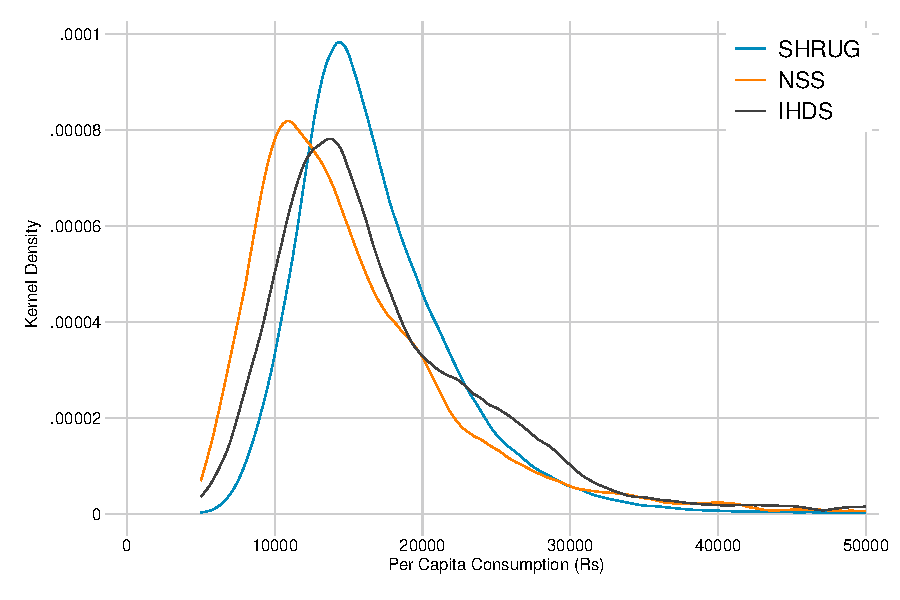
\includegraphics[scale=0.6]{\shrugpath/cons_compare_kdensity_rural} \\
    \panel{B. Urban} \\
    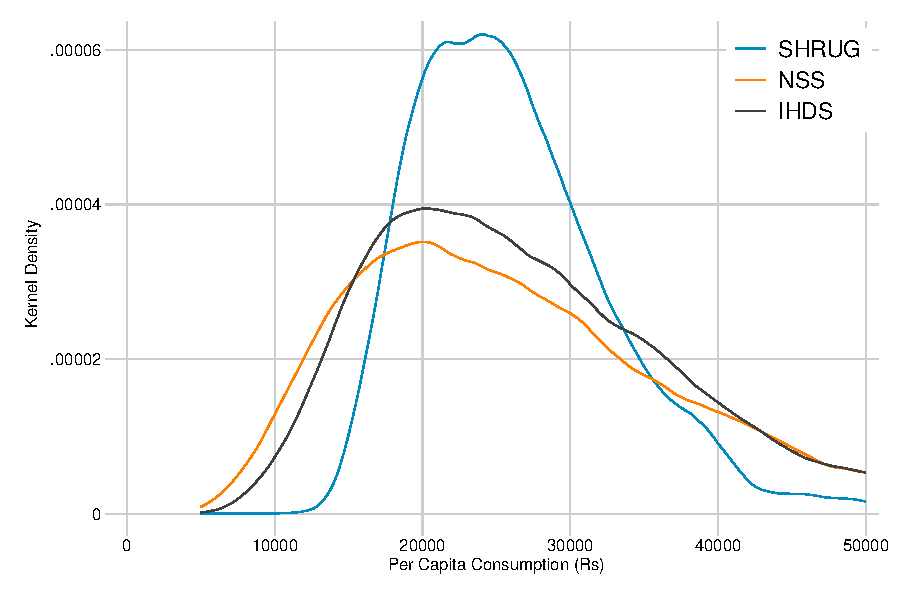
\includegraphics[scale=0.6]{\shrugpath/cons_compare_kdensity_urban} 
  \end{tabular}
\end{center}

\begin{adjustwidth}{2cm}{2cm}
  \footnotesize{\textit{Source}: Authors' analysis based on data in the
    \href{http://www.devdatalab.org/shrug}{Socioeconomic
      High-resolution Rural-Urban Geographic Dataset on India},
    National Sample Survey, and India Human Development
    Survey. \\ \textit{Note}: Figure~\ref{fig:ihds_nss_shrug_cons_kdensity} shows the
    distribution of location-level annual consumption per capita from the
    NSS, the IHDS, and SHRUG. Consumption in each location is a mean
    across households, calculated with sampling weights. Location
    units are PSUs in IHDS, FSUs in NSS, and towns or villages in
    SHRUG.}
\end{adjustwidth}

\label{fig:ihds_nss_shrug_cons_kdensity}
\end{figure}

%%%%%%%%%%%%%%%%%%%%%%%%%%%%%%%%
%% SHRUG vs. IHDS CONSUMPTION %%
%%%%%%%%%%%%%%%%%%%%%%%%%%%%%%%%
\newpage
\begin{figure}[H]\caption{District-level SHRUG Consumption vs. IHDS Consumption}
\begin{center}
  \begin{tabular}{c}
    \panel{A. Rural} \\
    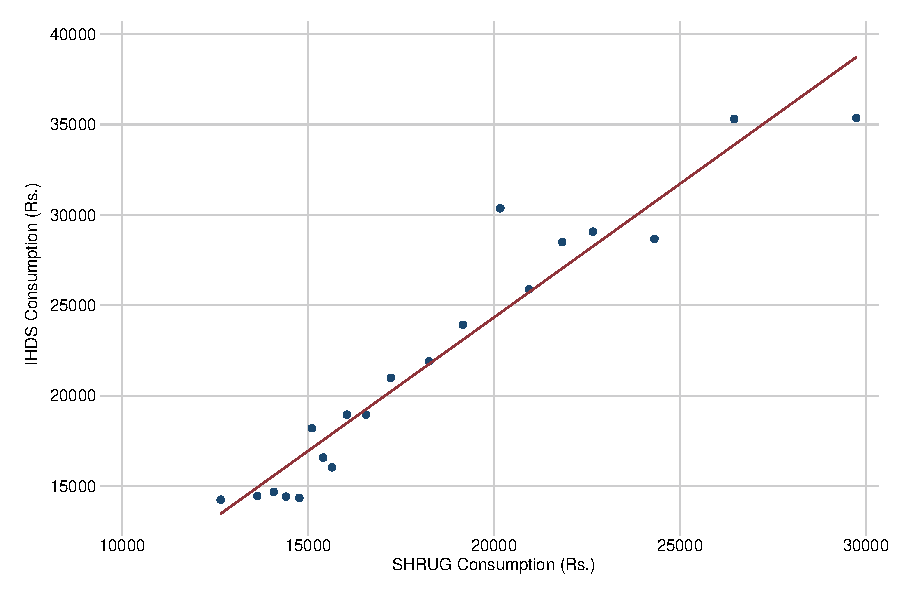
\includegraphics[scale=0.6]{\shrugpath/shrug_ihds_cons_comp_rural} \\
    \panel{B. Urban} \\
    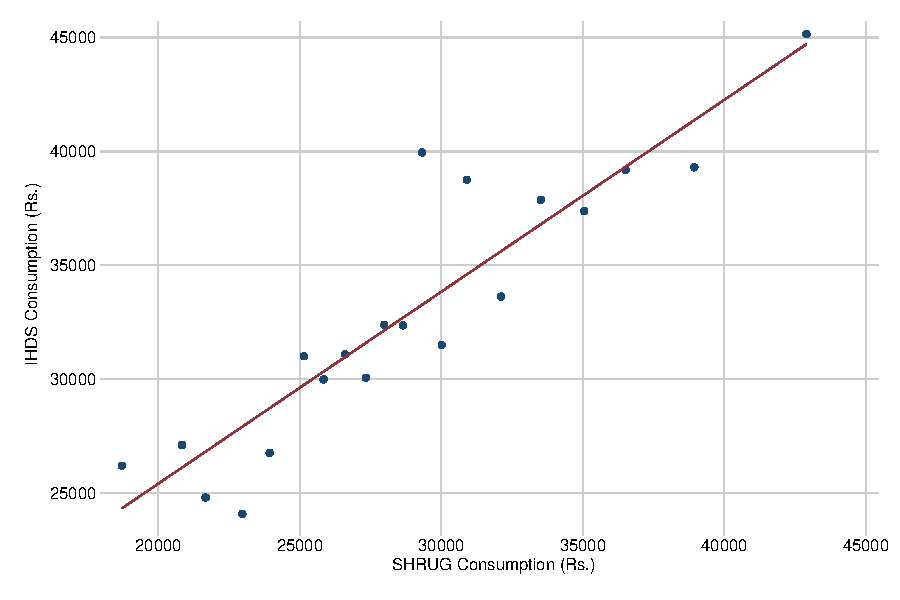
\includegraphics[scale=0.6]{\shrugpath/shrug_ihds_cons_comp_urban} \\
  \end{tabular}
\end{center}

\begin{adjustwidth}{2cm}{2cm}
\footnotesize{\textit{Source}: Authors' analysis based on data in the
  \href{http://www.devdatalab.org/shrug}{Socioeconomic High-resolution
    Rural-Urban Geographic Dataset on India} and India Human
  Development Survey. \\ \textit{Note}: Figure~\ref{fig:ihds_shrug_cons_binscatter} is a binned
  scatterplot of district-level average annual per capita consumption in the
  IHDS and the SHRUG, weighted by the count of individuals in each
  survey. The SHRUG sample has been restricted to the 331 districts where
  IHDS matches the Indian Population Census.}
\end{adjustwidth}

\label{fig:ihds_shrug_cons_binscatter}
\end{figure}

\newpage
\begin{figure}[H]\caption{Cross-sectional Night Lights vs. Development Proxies}
  \begin{center}
    \resizebox{\linewidth}{!}{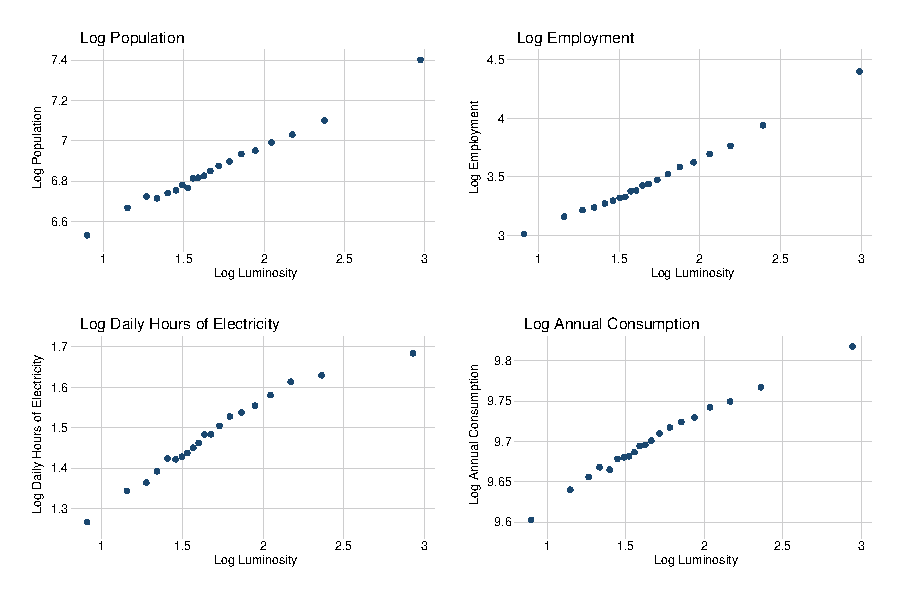
\includegraphics{\shrugpath/bins_lights_xvars}}
  \end{center}

\begin{adjustwidth}{2cm}{2cm}
  \footnotesize{\textit{Source}: Authors' analysis based on data in the
  \href{http://www.devdatalab.org/shrug}{Socioeconomic High-resolution
    Rural-Urban Geographic Dataset on India}. \\ \textit{Note}: Figure~\ref{fig:nl_xvars} shows the cross-sectional
    relationship between log night lights and log population (top
    left), log employment (top right), log hours of electricity
    (bottom left), and log annual consumption (bottom right). The
    graphs are generated by binscatter, which shows the mean Y
    variable in equally-dense bins across the distribution of log
    night lights. All graphs are run at the town/village level (except
    for log daily hours of electricity, which is only available for
    villages) and include district fixed effects.}
\end{adjustwidth}

\label{fig:nl_xvars}
\end{figure}

\begin{figure}[H]\caption{Cross-sectional Relationship between Night Lights and Development Proxies \cnewline as a Function of Electrification}
  \begin{center}
    \resizebox{\linewidth}{!}{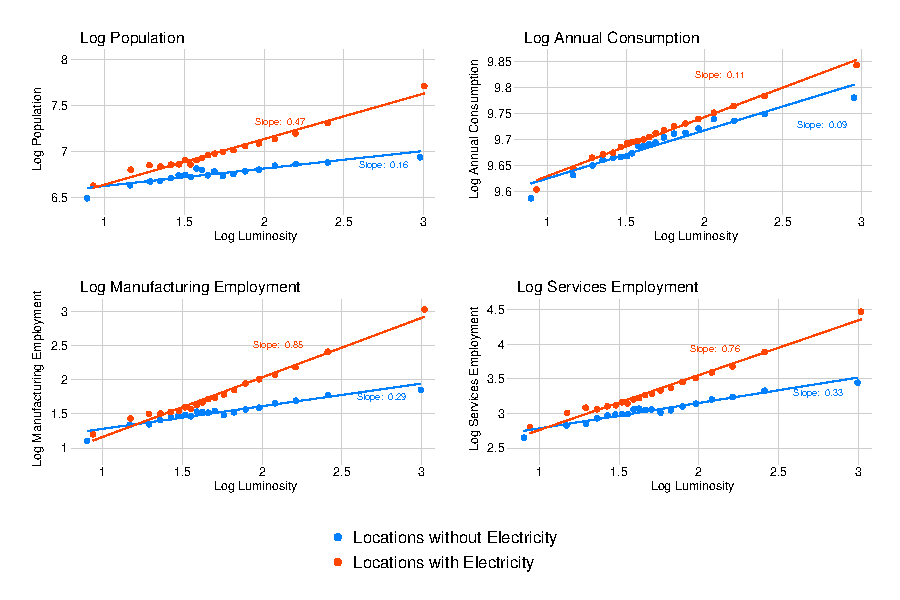
\includegraphics{\shrugpath/bins_lights_xvars_by_power}}
  \end{center}
  
  \begin{adjustwidth}{2cm}{2cm}
    \footnotesize{\textit{Source}: Authors' analysis based on data in
      the \href{http://www.devdatalab.org/shrug}{Socioeconomic
        High-resolution Rural-Urban Geographic Dataset on
        India}. \\ \textit{Note}: Figure~\ref{fig:nl_xvars_pow} shows the
      village/town-level cross-sectional relationship between four
      development proxies (population, annual consumption, manufacturing and
      services employment), with separate series' plotted for
      locations that do and do not report access to electricity. The
      graphs are generated by binscatter, which shows the mean Y
      variable in equally-dense bins across the distribution of log
      night lights. All graphs include district fixed effects.}
  \end{adjustwidth}
  
\label{fig:nl_xvars_pow}
\end{figure}

\newpage
\begin{figure}[H]\caption{Distribution of Job Density across Space}
  \begin{center}
    \resizebox{\linewidth}{!}{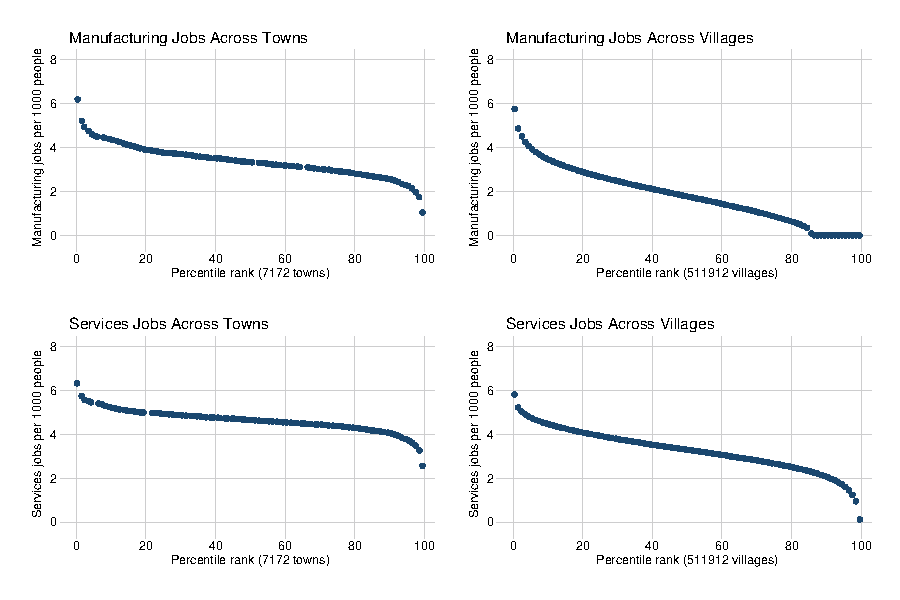
\includegraphics{\shrugpath/granular_job_distribution}}
  \end{center}

\begin{adjustwidth}{2cm}{2cm}
  \footnotesize{\textit{Source}: Authors' analysis based on data in the
  \href{http://www.devdatalab.org/shrug}{Socioeconomic High-resolution
    Rural-Urban Geographic Dataset on India} and Economic Census. \\ \textit{Note}: Figure~\ref{fig:job_dist} describes the distribution
    of non-farm jobs per 1000 people across villages and towns. The Y
    axes shows the log number of manufacturing- or service-sector jobs
    per 1000 people. The X axis shows the town or village rank on the
    same measure. The rank is population-weighted such that a village
    with rank 50 has more manufacturing or services jobs per 1000
    people than villages representing 50\% of the Indian
    population. Each point represents the mean of the measure in one
    percentile bin, or approximately either 70 towns or 5000
    villages.}

\end{adjustwidth}

\label{fig:job_dist}
\end{figure}

\newpage
\begin{figure}[H]\caption{Concentration of Poverty at Different Levels of Aggregation}
  \begin{center}
    \resizebox{\linewidth}{!}{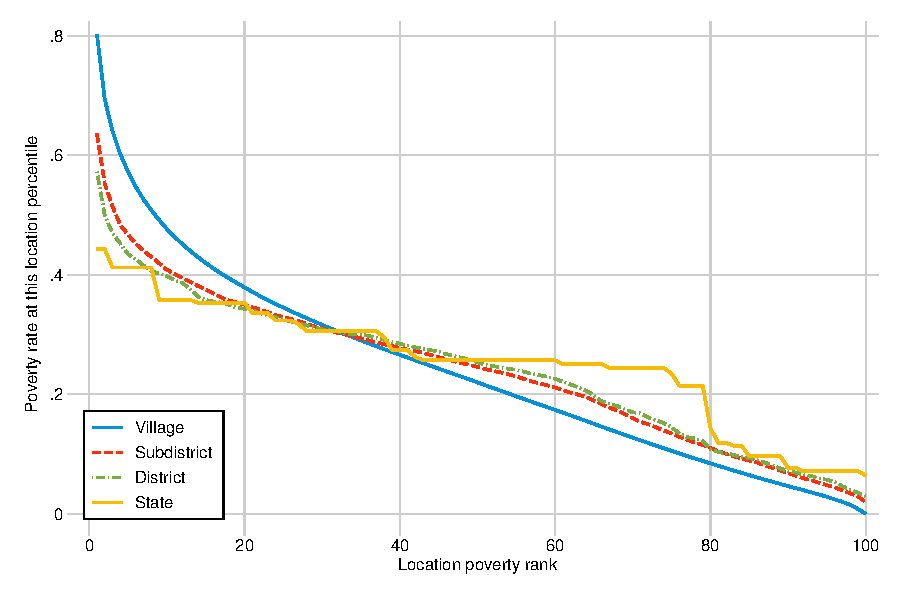
\includegraphics{\shrugpath/pov_rate_perc_loc}}
  \end{center}

\begin{adjustwidth}{2cm}{2cm}
  \footnotesize{\textit{Source}: Authors' analysis based on data in the
  \href{http://www.devdatalab.org/shrug}{Socioeconomic High-resolution
    Rural-Urban Geographic Dataset on India}. \\ \textit{Note}: Figure~\ref{fig:pov_dist} plots locations' average
    poverty rates against their poverty rate ranking. The four data
    series' represent four different level of aggregation: state
    (n=35), district (n=600), subdistrict (n=5600), and village/town
    (n=590,000). The graph shows, for instance, that the poverty rate
    in the 5th percentile district is 37\%, while the poverty rate in
    the 5th percentile village is 50\%.}

\end{adjustwidth}

\label{fig:pov_dist}
\end{figure}


\end{appendix}

\end{document}
